\documentclass[twoside,a4paper,english,11pt]{book}

\usepackage{hyperref}
\usepackage{fontenc}
\usepackage[latin9]{inputenc}
\usepackage{url}
\usepackage{epsfig} % permet posar figures amb format .eps
\usepackage{subfigure} % permet fer subfigures
\usepackage{setspace} % permet canviar l'espai interlinial
\usepackage{tocbibind} % posa la bibliografia a la TOC
\usepackage{a4wide}
\usepackage{fullpage}
\usepackage{verbatim}
\usepackage{color}
\usepackage{calc}
\usepackage[table]{xcolor}
\usepackage{pdflscape}
\usepackage{fancyvrb}
\usepackage{amsfonts}
\usepackage{listings}

\definecolor{lightgray}{rgb}{0.75,0.75,0.75}
\definecolor{tabbg1}{rgb}{0.85,0.85,0.85}
\definecolor{tabfg1}{rgb}{0.0,0.0,0.0}
\definecolor{tabbg2}{rgb}{0.95,0.95,0.95}
\definecolor{tabfg2}{rgb}{0.0,0.0,0.0}

\usepackage{makecell}
\newlength\hrulethickness
\setlength\hrulethickness{1.75\arrayrulewidth}
\newcommand{\hlinethick}{\Xhline{\hrulethickness}}
\lstset{framerule=\hrulethickness}


\newcommand{\EXTRAE}{\textsf{{E}xtrae}}
\newcommand{\PARAVER}{\textsf{{P}araver}}
\newcommand{\FOLDING}{\textsf{{F}olding}}

\newcommand{\FOLDINGVERSION}{1.0rc8}


\def\graybox#1{
  \medskip
  \colorbox{lightgray}{
    \begin{minipage}[t]{0.95\textwidth}
    #1
    \end{minipage}
   }
}

\urlstyle{leostyle}

\begin{document}

\pagenumbering{roman}

\title{\FOLDING \\
       User guide manual\\
       for version \FOLDINGVERSION}
\author{
tools@bsc.es
}

\maketitle
\tableofcontents
\listoffigures
\listoftables


\chapter{User guide}\label{cha:UserGuide}

\section{Quick start guide}

\let\oldv\verbatim
\let\oldendv\endverbatim

\def\verbatim{\par\setbox0\vbox\bgroup\oldv}
\def\endverbatim{\oldendv\egroup\fboxsep0pt \noindent\colorbox[gray]{0.8}{\usebox0}\par}


The \FOLDING is a mechanism that provides instantaneous performance metrics, source code references and memory references\footnote{This last option is experimental at the moment of writing this document}.
This mechanism receives a trace-file (currently generated by \EXTRAE - see further details on generating a trace-file for the \FOLDING in Appendix~\ref{cha:GetATrace}) and generates plots and an additional trace-file depicting the fine evolution of the performance.
The \FOLDING uses information captured through instrumentation and sampling mechanisms and smartly combines them.
In this context, the samples are gathered from scattered computing regions into a synthetic region by preserving their relative time within their original region so that the sampled information determines how the performance evolves within the region.
Consequently, the folded samples represent the progression in shorter periods of time no matter the monitoring sampling frequency, and also, the longer the runs the more samples get mapped into the synthetic instance.
The framework has shown mean differences up to 5\% when comparing results obtained sampling frequencies that are two orders of magnitude more frequent.

\subsection{Decompressing the package}

The \FOLDING package is distributed in a .tar.bz2 file that can be uncompressed in the working directory by executing the following command:

\begin{verbatim}
# tar xvz folding-1.0rc8-x86_64.tar.bz2
\end{verbatim}

where \texttt{folding-1.0rc8-x86\_64.tar.bz2} refers to the \FOLDING package as distributed from the BSC web page\footnote{\url{http://www.bsc.es/computer-sciences/performance-tools/downloads}}.

\subsection{Contents of the package}\label{subsec:ContentsOfInstallation}

After decompressing the package, the working directory should be populated with the directories (and corresponding descriptions) as listed in Table~\ref{tab:contents_folding_package}.

\begin{table}
  \small
  \begin{center}
  \rowcolors{2}{tabbg2}{tabbg1}
  \caption{Contents of the folding package.}
  \label{tab:contents_folding_package}
    \begin{tabular}{l c l}
    \hlinethick
    Directory & & Contents \\
    \hline
    bin/ & & Binary packages \\
    etc/ & & \\
    \ \ extrae-configurations/ & & Minimal configuration files for \EXTRAE \\
    \ \ models/ & & Configuration files to calculate performance models \\
    \ \ \ \ basic/ & & \\
    \ \ \ \ ibm-power5/ & & \\
    \ \ \ \ ibm-power7/ & & \\
    \ \ \ \ ibm-power8/ & & \\
    \ \ \ \ intel-haswell/ & & \\
    \ \ \ \ intel-nehalem/ & & \\
    \ \ \ \ intel-sandybridge/ & & \\
    include/ & & Header files for the development of 3rd party tools \\
    lib/ & & Libraries for the folding \\
    share/ & & Miscellaneous files \\
    \ \ cfg/ & & Configuration files for Paraver \\
    \ \ doc/ & & Documentation\\
    \ \ \ \ html & & \\
    \ \ examples/ & & \\
    \ \ \ \ folding-writer/ & & Example on how to generate data for the folding \\
    \ \ \ \ user-functions/ & & Sample tracefile with manually instrumented regions \\
    \ \ \ \ clusters/ & & Sample tracefile with automatically detected regions \\
    \hlinethick
    \end{tabular}
  \end{center}
\end{table}


\subsection{Quick run}

This section provides examples of two types of execution of the \FOLDING tool.
These examples take benefit of the included sample trace-files from the package.
For further information on how to generate trace-files for the \FOLDING tool, check Appendix~\ref{cha:GetATrace}.

\subsubsection{Applied to manually instrumented regions}\label{subsubsec:ManualExample}

This first example uses a trace-file from the 444.namd SPEC benchmark that contains manually instrumented information that is located in 

\begin{verbatim}
${FOLDING_HOME}/etc/share/examples/user-functions
\end{verbatim}

This trace-file was generated by \EXTRAE and delimiting the main loop using the \EXTRAE API\footnote{Please refer to \url{http://www.bsc.es/computer-sciences/performance-tools/documentation} for the latest \EXTRAE User's Guide.}, more precisely the \texttt{Extrae\_user\_function} which emits events with label \texttt{User function} (or event type 60000019).
To apply the \FOLDING process to this trace-file, simply execute the following commands:

\begin{verbatim}
# cd ${FOLDING_HOME}/etc/share/examples/user-functions
# ${FOLDING_HOME}/bin/folding 444.namd.prv "User function"
\end{verbatim}

\subsubsection{Applied to automatically characterized regions}\label{subsubsec:ClusteredExample}

This example consists of a trace-file for the Nemo application when executed in MareNostrum3.
This trace-file contains information regarding automatically characterized regions.
This characterization has been done using the Clustering tool\footnote{Please refer to \url{http://www.bsc.es/computer-sciences/performance-tools/documentation} for the latest documentation with respect to the Clustering tool.}.
This tool enriches the trace-file by adding events labeled as \texttt{Cluster ID} (and event type 90000001) into the trace-file.
In this context, these events identify similar computation regions based on the event value.
To apply the \FOLDING process to this trace-file, simply execute the following commands:

\begin{verbatim}
# cd ${FOLDING_HOME}/etc/share/examples/user-functions
# ${FOLDING_HOME}/bin/folding \
  nemo.exe.128tasks.chop1.clustered.prv "Cluster ID"
\end{verbatim}

This trace-file also contains all the necessary performance counters in order to take benefit of several performance models based on performance counters.
Simply add the \texttt{-model intel-sandybridge} option to the \FOLDING script to generate the plots with information of the models instead of providing each performance counter individually.
The commands to execute should look like this:

\begin{verbatim}
# cd ${FOLDING_HOME}/etc/share/examples/user-functions
# ${FOLDING_HOME}/bin/folding -model intel-sandybridge \
  nemo.exe.128tasks.chop1.clustered.prv "Cluster ID"
\end{verbatim}

\subsection{Exploring the results}

The \FOLDING mechanism generates two types of output inside a directory named as the trace-file given (without the \texttt{.prv} suffix).
The first type of results include a set of gnuplot files where each of these represents the evolution of the performance counters within the region.
The tool also generates a \PARAVER trace-file with synthetic information derived from the \FOLDING mechanism.

\subsubsection{Using gnuplot}

With respect to the gnuplot files, the \FOLDING mechanism generates as many files as the combination of analyzed regions (clusters, OpenMP outlined routines, taskified OmpSs routines, or manually delimited regions) and the counters gathered during the application execution.
The user can easily list the generated gnuplot files calling \texttt{ls *.gnuplot} within the directory created.
The name of the gnuplot files contain the trace-file prefix, the identification of the region folded, and the performance counter shown.
For instance, the example described in Section~\ref{subsubsec:ManualExample} generates output files that can be explored by executing the command:

\begin{verbatim}
# gnuplot -persist \
  444.namd.codeblocks.fused.any.any.any.main.Group_0.PAPI_TOT_INS.\
  gnuplot
\end{verbatim}

When executing the aforementioned command, the \texttt{gnuplot} command should open a window that resembles that in Figure~\ref{fig:444_namd_instructions}\footnote{Warning! If the user has problems to open the gnuplot, they should check whether the gnuplot installation is compatible and supports the default terminal. Otherwise, simply select the appropriate terminal (or leave it blank) in the first four lines in the gnuplot script}.
The Figure shows that the application faces six phases that execute at 4,500~MIPS approximately.
Most of the code occurs in three code locations (being line 76 the most observed line), and we also observe that phases related to high MIPS are related with the activity in the middle of the code-line plot.

\begin{figure}
  \centering
  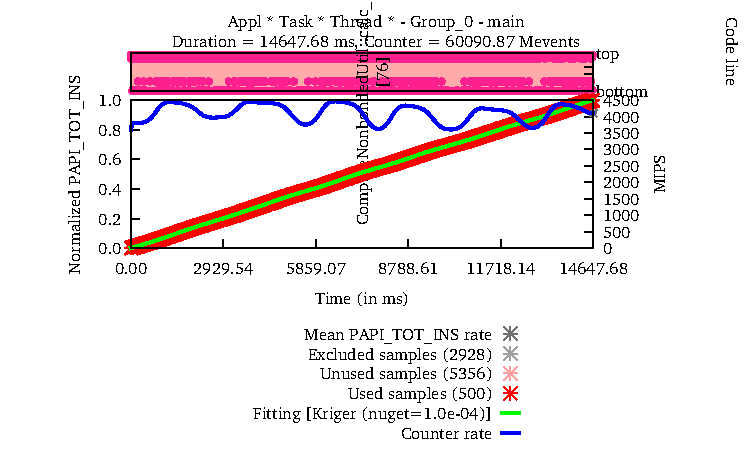
\includegraphics[width=0.65\textwidth]{figures/user-guide/444_namd_tot_ins.pdf}
  \caption{Evolution of graduated instructions for 444.namd.}
  \label{fig:444_namd_instructions}
\end{figure}


This file refers to the user routine \texttt{main} (which was manually instrumented) of the trace-file 444.namd.prv and provides information of the total graduated instructions (\texttt{PAPI\_TOT\_INS}). 
The user will notice that there are additional files for the different performance counters and they can explore them individually.
The \FOLDING also generates an additional plot that combines the metrics of all the counters into a single plot.
This plot mainly provides information with respect to the MIPS rate (referenced on the right Y-axis), and ratio of the remaining performance counters per instruction (referenced on the left Y-axis).
For the particular case of the example from Section~\ref{subsubsec:ManualExample}, this plot can be explored calling:

\begin{verbatim}
# gnuplot -persist \
  444.namd.codeblocks.fused.any.any.any.main.\
  Group_0.ratio_per_instruction.gnuplot
\end{verbatim}

This command should generate an output combining all the performance counter slopes as shown in Figure~\ref{fig:444_namd_ratio_per_instruction}.

\begin{figure}
  \centering
  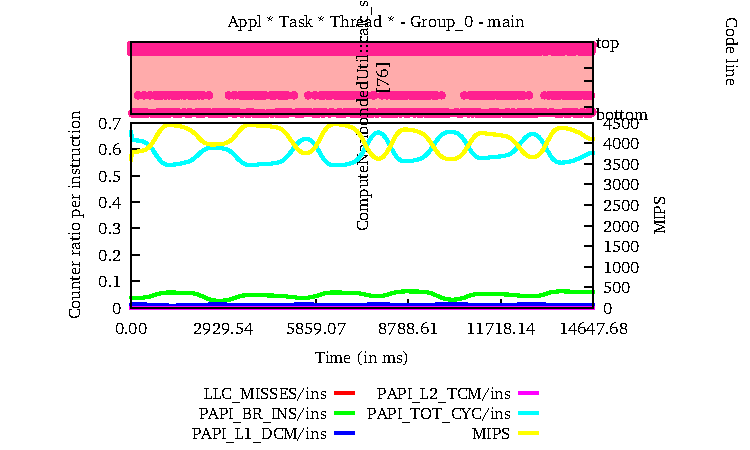
\includegraphics[width=0.65\textwidth]{figures/user-guide/444_namd_ratio_per_instruction.pdf}
  \caption{Evolution of multiple counters for 444.namd.}
  \label{fig:444_namd_ratio_per_instruction}
\end{figure}


The aforementioned instructions also apply to the automatically delimited example described in Section~\ref{subsubsec:ClusteredExample}.
In this case, the region names are numbered as \texttt{Cluster\_1} to \texttt{Cluster\_11}, but they also contain the trace-file prefix and the performance counters to explore them individually.
If the user requested the performance models, then additional gnuplot files are created to provide information regarding these models.
For the particular case of the Intel SandyBridge model, it generates three models that always generate the MIPS rate and add different metrics:

\begin{itemize}
	\item \textit{instruction-mix}\\
	Gives insight of the type of instructions executed along the region.
	\item \textit{architecture-impact}\\
	Provides information regarding to the cache misses at different levels and the branch mispredicts along the region.
	\item \textit{stall-distribution}\\
	This plot shows information regarding on which components of the processor are stalling the processor pipeline.
\end{itemize}

For instance, to open the instruction mix for the region labeled as Cluster 1 of the Nemo application executed in Section~\ref{subsubsec:ClusteredExample}, the user needs to open the plot invoking the commands below and should obtain a plot similar to Figure~\ref{fig:Nemo_cluster1_instructionmix}.
The reader may see that the application shows two distinctive phases (green and blue) and within each of them there are two repetitions of the same performance.

\begin{verbatim}
# gnuplot -persist \
  nemo.exe.128tasks.chop1.clustered.codeblocks.fused.any.any.any.\
  Cluster_1.Group_0.instructionmix.gnuplot
\end{verbatim}

\begin{figure}
  \centering
  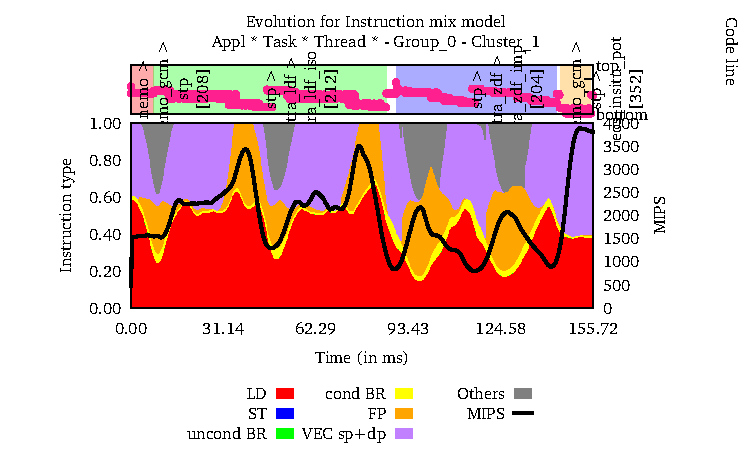
\includegraphics[width=0.65\textwidth]{figures/user-guide/nemo_cluster1_instructionmix.pdf}
  \caption{Instruction mix decomposition for Cluster 1 of Nemo.}
  \label{fig:Nemo_cluster1_instructionmix}
\end{figure}


The tool also provides a GUI-based tool to explore the plots. 
the user may invoke a visualizer named \texttt{wxfolding-viewer}, by invoking it from the newly created directory such as:

\begin{verbatim}
# ${FOLDING_HOME}/bin/wxfolding-viewer *.wxfolding
\end{verbatim}

\subsubsection{Using Paraver}

The \FOLDING process generates a trace-file with a suffix \texttt{.folded.prv} that lets \PARAVER to display some parts of the folded results.
The \FOLDING package includes several configuration files in the \texttt{\$\{FOLDING\_HOME\}/share/cfg} directory for \PARAVER to help analysing the results.
From the configuration files contained in that directory, we outline the following:

\begin{itemize}
	\item \textit{views}/
	\begin{itemize}
		\item \texttt{win\_folded\_type.cfg}\\
		Generates a time-line that shows in which instances the \FOLDING results have been integrated. This helps correlating the original trace-file and its contents with the folded trace-file. Notice that only one instance per type (where type refers to function, cluster, \textit{etc...}) is folded.
		\item \texttt{win\_folded\_mips.cfg}\\
		Generates a time-line showing a signal of the MIPS rate within the folded instances. See in Figure~\ref{fig:444_namd_instructions_paraver} a time-line depicting the MIPS rate achieved in the example trace-file for 444.namd.
		\item \texttt{win\_folded\_processed\_call-stack\_caller.cfg}\\
		Generates a time-line showing the most time-dominant routines as they have been executed within the folded instances. Figure~\ref{fig:Nemo_cluster1_callers_paraver} shows a time-line depicting the called routines for the Nemo example.
		\item \texttt{win\_folded\_processed\_call-stack\_callerline.cfg}\\
		Generates a time-line showing the most time-dominant source code references (as pair of line and file) as they have been executed within the folded instances.
	\end{itemize}
	\item \textit{histograms}/
	\begin{itemize}
		\item \texttt{3dh\_folded\_mips\_per\_caller.cfg}\\
		Generates a histogram that shows the achieved MIPS rate depending on the caller (columns) for a particular region folded.
		\item \texttt{3dh\_folded\_mips\_per\_callerline.cfg}\\
		Generates a histogram that shows the achieved MIPS rate depending on the source code references (pair of line and file in columns) for a particular region folded.
	\end{itemize}
\end{itemize}

\begin{figure}
  \centering
  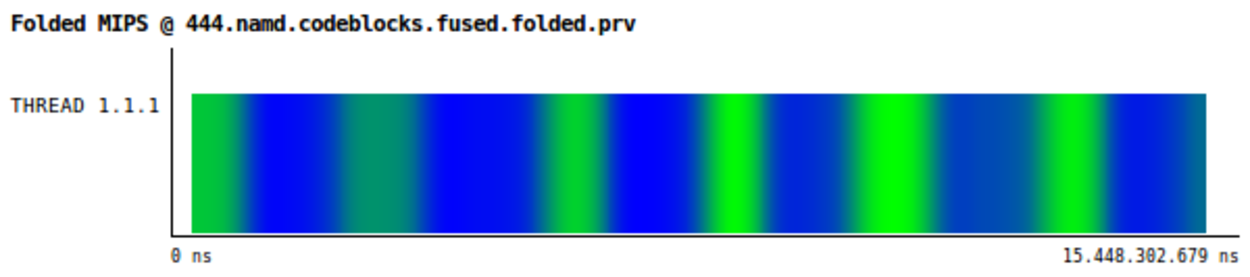
\includegraphics[width=0.75\textwidth]{figures/user-guide/444_namd_tot_ins_paraver.pdf}
  \caption{Evolution of graduated instructions for 444.namd in Paraver.}
  \label{fig:444_namd_instructions_paraver}
\end{figure}


\begin{figure}
  \centering
  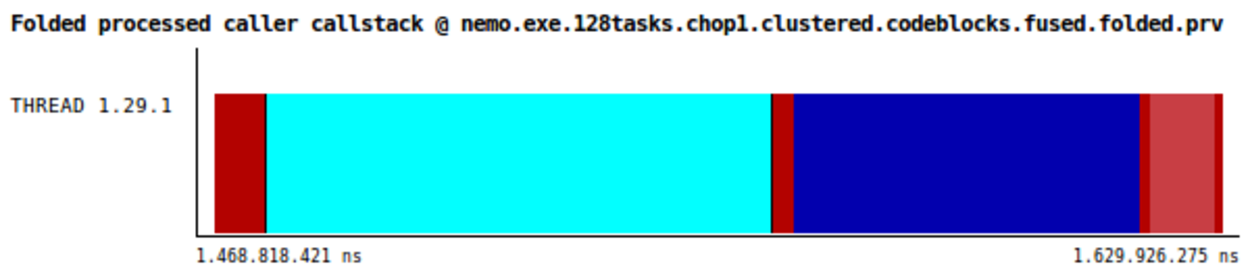
\includegraphics[width=0.75\textwidth]{figures/user-guide/nemo_cluster1_caller_paraver.pdf}
  \caption{Paraver time-line showing the callers for Cluster 1 of Nemo.}
  \label{fig:Nemo_cluster1_callers_paraver}
\end{figure}


\section{Configuration, build and installation}

This section describes how to build and install the \FOLDING package.
The \FOLDING package (and its dependencies) requires the Boost library (only the headers suffice), a C compiler, a Fortran compiler and a C++ compiler that supports the C++ 2011 specification (such as g++ version 4.8).
This package optionally uses the \texttt{strucchange} package from the R statistical application (and may execute in parallel if the \texttt{doParallel} is available) to use the piece-wise linear regression interpolation mechanism.
Additionally, the \FOLDING package requires the libtools package to be installed.
This package helps on the parsing of Paraver trace-files and can be downloaded from the BSC download web page.

\subsection{Libtools package}~\label{subsec:LibtoolsInstallation}

This package can be downloaded from the BSC web page and requires the boost header files\footnote{The libtools package has been successfully tested against version from 1.48 to 1.54.}.
If the boost header files are located in the system's default, simply run the following command:

\begin{verbatim}
# ./configure --prefix=/home/harald/aplic/libtools/1.0 \
  && make && make install
\end{verbatim}

where \texttt{--prefix} indicates the destination folder for this package.

If the boost header files are located elsewhere in the system, run the following command:

\begin{verbatim}
# ./configure --prefix=/home/harald/aplic/libtools/1.0 \
  --with-boost=/path/to/boost \
  && make && make install
\end{verbatim}

\subsection{Folding package}

The most basic configuration for the \FOLDING package honors the following commands:

\begin{verbatim}
# ./configure --with-libtools=$HOME/aplic/libtools/1.0 \
  --prefix=$HOME/aplic/folding/1.0rc8 && \
  make && make install
\end{verbatim}

where \texttt{--with-libtools} refers to the location of the libtools package installed in Section~\ref{subsec:LibtoolsInstallation} and \texttt{--prefix} indicates where to install the \FOLDING tool.
If the compilation and installation succeed, the contents of the target installation should look like as the contents defined in Section~\ref{subsec:ContentsOfInstallation}.

The \FOLDING tool supports several compilation flags that modify the behavior or enable additional functionalities of the tool.
The following list groups the flags according to the behavior they enable.

\begin{itemize}

	\item \texttt{--with-clustering-suite=<DIR>}\\
    The \FOLDING tool relies on the similarity between the folded instances in order to generate its results. By default, the \FOLDING tool includes two mechanisms to reduce the noise that appear from using instances with significant different behavior. However, this flag allows using the BSC Clustering suite as a third alternative in order to reduce the noise.

	\item \texttt{--with-R=<DIR1>, --with-cube=<DIR2>, --with-clang=<DIR3>}\\
	Enables the usage of piece-wise linear regressions on top of the strucchange package\footnote{\url{http://cran.r-project.org/web/packages/strucchange/index.html}} from the R statistical application\footnote{\url{http://www.r-project.org}}. This functionality requires the clang compiler\footnote{\url{http://clang.llvm.org}} and can generate input files for the Cube3 performance analysis package\footnote{\url{http://www.scalasca.org/software/cube-3.x/download.html}}.

	\item \texttt{--with-boost=<DIR>}\\
	This flag lets the \FOLDING to use a given Boost installation package.

	\item \texttt{--enable-gui}\\
	The results of the \FOLDING tool is a set of gnuplot files that have to explored manually. If this flag is given at the configure step, the \FOLDING package would include a GUI written in Python that helps exploring all the results from the tool.

	\item \texttt{--enable-callstack-analysis}\\
	This flag enables the call-stack analysis of the segments captured during the measurement step. Enabling this option results in gnuplot files that depict the performance progression collocated with the source code progression.

	\item \texttt{--enable-reference-analysis}\\
	This flag enables the memory references analysis of the references captured during the measurement step (currently, through the \texttt{perf} system tool). Enabling this option results in gnuplot files that depict the performance progression collocated with the memory address space and the sampled references.

\end{itemize}


\chapter{Generate a trace-file for the Folding}\label{cha:GetATrace}

This chapter covers the minimum and necessary steps so as to configure \EXTRAE\footnote{Please refer to \url{http://www.bsc.es/computer-sciences/performance-tools/documentation} for the latest \EXTRAE User's Guide.} in order to use its resulting trace-files for the Folding process.
There are three requirements when monitoring an application with \EXTRAE in order to take the most benefit from the \FOLDING tool. 
First, it is necessary to enable the sampling mechanism in addition to the instrumentation mechanism (see Section~\ref{sec:EnableSamplingMechanism}).
Second, it is convenient to collect the appropriate performance counters for the underlying processor (see Section~\ref{sec:CollectingAppropriatePerformanceCounters}).
Finally, \EXTRAE needs to capture a segment of the call-stack in order to allow the \FOLDING to provide information regarding the progression of the executed routines.
The forthcoming sections provide information on how to enable these functionalities through the XML tags for the \EXTRAE configuration file.

\section{Enabling the sampling mechanism}\label{sec:EnableSamplingMechanism}

\EXTRAE is an instrumentation package that by default collects information from different parallel runtimes, including but not limited to: MPI, OpenMP, pthreads, CUDA and OpenCL (and even combinations of them).
\EXTRAE can be configured so that it also uses sampling mechanisms to capture performance metrics on a periodic basis.
There are currently two alternatives to enable sampling in \EXTRAE: using alarm signals and using performance counters.
For the sake of simplicity, this document only covers the alarm-based sampling.
However, if the reader would like to enable the sampling using the performance counters they must look at section 4.9 in the \EXTRAE User's Manual for more details.

\begin{lstlisting}[
 float=h,
 language=XML,
 frame=tb,
 basicstyle=\small\ttfamily,
 keywordstyle=\small\bfseries,
 commentstyle=\small\itshape,
 numbers=left,
 firstnumber=1,
 numberstyle=\tiny\color{gray},
 captionpos=t,
 caption={Enable default time-based sampling in Extrae.},
 label=lst:Extrae_enable_sampling_basic,
]
<sampling enabled="yes" type="default" period="50m" variability="10m"/>
\end{lstlisting}


The XML statements in Listing~\ref{lst:Extrae_enable_sampling_basic} need to be included in the \EXTRAE configuration file.
These statements indicate \EXTRAE that sampling is enabled (\texttt{enabled="yes"}).
They also tell \EXTRAE to capture samples every 50~milliseconds (ms) with a random variability of 10~ms, that means that samples will be randomly collected with a periodicity of $50{\pm}10$~ms.
With respect to type, it determines which timer domain is used (see {\tt man 2 setitimer} or {\tt man 3p setitimer} for further information on time domains).
Available options are: {\tt real} (which is also the {\tt default} value, {\tt virtual} and {\tt prof} (which use the SIGALRM, SIGVTALRM and SIGPROF respectively).
The default timing accumulates real time, but only issues samples at master thread.
To let all the threads collect samples, the type must be set to either {\tt virtual} or {\tt prof}.

Additionally, the \FOLDING mechanism is able to combine several performance models and generate summarized results that simplify understanding the behavior of the node-level performance.
Since these performance models are heavily-tighted with the performance counters available on each processor architecture and family, the following sections provide \EXTRAE XML configuration files ready to use on several architectures.
Since each architecture has different characteristics, the user may need to tune the XML presented there to make sure that all the list performance counters are gathered appropriately.

\section{Collecting the appropriate performance counters}\label{sec:CollectingAppropriatePerformanceCounters}

The \FOLDING mechanism provides, among other type of information, the progression of performance metrics along a delimited region through instrumentation points.
These performance metrics include the progression of performance counters of every performance counter by default.
To generate these kind of reports, \EXTRAE must collect the performance counters during the application execution and this is achieved by defining counter sets into the \texttt{<counters>} section of the \EXTRAE configuration file (see Section 4.19 of the \EXTRAE User's guide for more information).

There has been research that has developed some performance models based on performance counters ratios among performance counters in order to ease the analysis of the reports.
Each of these performance models aims at providing insight of different aspects of the application and system during the execution.
Since the availability of the performance counters changes from processor to processor (even in the same processor family), the following sections describe the performance counters that are meant to be collected in order to calculate these performance models.
These sections include the minimal \texttt{<counters>} sections to be added in a previously existing \EXTRAE configuration file, but the \FOLDING package also includes full \EXTRAE configuration files in \texttt{\$\{FOLDING\_HOME\}/etc/extrae-configurations}.

\subsection{Intel Haswell processors}

\begin{lstlisting}[
 float=h,
 language=XML,
 frame=tb,
 basicstyle=\small\ttfamily,
 keywordstyle=\small\bfseries,
 commentstyle=\small\itshape,
 numbers=left,
 firstnumber=1,
 numberstyle=\tiny\color{gray},
 captionpos=t,
 caption={Counter definition sets for the Extrae configuration file when used on Intel Haswell procesors.},
 label=lst:Extrae_counters_intel_haswell,
]
<cpu enabled="yes" starting-set-distribution="cyclic">
  <set enabled="yes" domain="all" changeat-time="500000us">
    PAPI_TOT_INS,PAPI_TOT_CYC,PAPI_L1_DCM,PAPI_L2_DCM
  </set>
  <set enabled="yes" domain="all" changeat-time="500000us">
    PAPI_TOT_INS,PAPI_TOT_CYC,PAPI_L3_TCM,RESOURCE_STALLS:SB,RESOURCE_STALLS:ROB
  </set>
  <set enabled="yes" domain="all" changeat-time="500000us">
    PAPI_TOT_INS,PAPI_TOT_CYC,PAPI_SR_INS,PAPI_BR_CN,PAPI_BR_UCN
  </set>
  <set enabled="yes" domain="all" changeat-time="500000us">
    PAPI_TOT_INS,PAPI_TOT_CYC,PAPI_BR_MSP,PAPI_LD_INS
  </set>
  <set enabled="yes" domain="all" changeat-time="500000us">
    PAPI_TOT_INS,PAPI_TOT_CYC,RESOURCE_STALLS,RESOURCE_STALLS:RS
  </set>
</cpu>
\end{lstlisting}


The listing~\ref{lst:Extrae_counters_intel_haswell} indicates \EXTRAE to arrange five performance counter sets with performance counters that are available on Intel Haswell processors.
The collection of these performance counters allows the \FOLDING to apply the models contained in the \texttt{\$\{FOLDING\_HOME\}/etc/models/intel-sandybridge} that include: instruction mix, architecture impact and stall distribution.
Unfortunately, the PMU of the Intel Haswell processors do not count neither floating point nor vector instructions.

\subsection{Intel SandyBridge processors}

\begin{lstlisting}[
 float=h,
 language=XML,
 frame=tb,
 basicstyle=\small\ttfamily,
 keywordstyle=\small\bfseries,
 commentstyle=\small\itshape,
 numbers=left,
 firstnumber=1,
 numberstyle=\tiny\color{gray},
 captionpos=t,
 caption={Counter definition sets for the Extrae configuration file when used on Intel SandyBridge procesors.},
 label=lst:Extrae_counters_intel_sandybridge,
]
<cpu enabled="yes" starting-set-distribution="cyclic">
  <set enabled="yes" domain="all" changeat-time="500000us">
    PAPI_TOT_INS,PAPI_TOT_CYC,PAPI_L1_DCM,PAPI_L2_DCM,PAPI_L3_TCM
  </set>
  <set enabled="yes" domain="all" changeat-time="500000us">
    PAPI_TOT_INS,PAPI_TOT_CYC,PAPI_BR_MSP,PAPI_BR_UCN,PAPI_BR_CN,RESOURCE_STALLS
  </set>
  <set enabled="yes" domain="all" changeat-time="500000us">
    PAPI_TOT_INS,PAPI_TOT_CYC,PAPI_VEC_DP,PAPI_VEC_SP,PAPI_FP_INS
  </set>
  <set enabled="yes" domain="all" changeat-time="500000us">
    PAPI_TOT_INS,PAPI_TOT_CYC,PAPI_LD_INS,PAPI_SR_INS
  </set>
  <set enabled="yes" domain="all" changeat-time="500000us">
    PAPI_TOT_INS,PAPI_TOT_CYC,RESOURCE_STALLS:LOAD,RESOURCE_STALLS:STORE,
    RESOURCE_STALLS:ROB_FULL,RESOURCE_STALLS:RS_FULL
  </set>
</cpu>
\end{lstlisting}


The listing~\ref{lst:Extrae_counters_intel_sandybridge} indicates \EXTRAE to configure five performance counter sets with performance counters that are available on Intel SandyBridge processors.
The collection of these performance counters allows the \FOLDING to apply the models contained in the \texttt{\$\{FOLDING\_HOME\}/etc/models/intel-sandybridge} that include: instruction mix, architecture impact and stall distribution.

\subsection{Intel Nehalem processors}

\begin{lstlisting}[
 float=h,
 language=XML,
 frame=tb,
 basicstyle=\small\ttfamily,
 keywordstyle=\small\bfseries,
 commentstyle=\small\itshape,
 numbers=left,
 firstnumber=1,
 numberstyle=\tiny\color{gray},
 captionpos=t,
 caption={Counter definition sets for the Extrae configuration file when used on Intel SandyBridge procesors.},
 label=lst:Extrae_counters_intel_sandybridge,
]
<cpu enabled="yes" starting-set-distribution="cyclic">
  <set enabled="yes" domain="all" changeat-time="500000us">
    PAPI_TOT_INS,PAPI_TOT_CYC,PAPI_L1_DCM,PAPI_L2_DCM,PAPI_L3_TCM
  </set>
  <set enabled="yes" domain="all" changeat-time="500000us">
    PAPI_TOT_INS,PAPI_TOT_CYC,PAPI_BR_MSP,PAPI_BR_UCN,PAPI_BR_CN,RESOURCE_STALLS
  </set>
  <set enabled="yes" domain="all" changeat-time="500000us">
    PAPI_TOT_INS,PAPI_TOT_CYC,PAPI_VEC_DP,PAPI_VEC_SP,PAPI_FP_INS
  </set>
  <set enabled="yes" domain="all" changeat-time="500000us">
    PAPI_TOT_INS,PAPI_TOT_CYC,PAPI_LD_INS,PAPI_SR_INS
  </set>
  <set enabled="yes" domain="all" changeat-time="500000us">
    PAPI_TOT_INS,PAPI_TOT_CYC,RESOURCE_STALLS:LOAD,RESOURCE_STALLS:STORE,
    RESOURCE_STALLS:ROB_FULL,RESOURCE_STALLS:RS_FULL
  </set>
</cpu>
\end{lstlisting}


The listing~\ref{lst:Extrae_counters_intel_nehalem} indicates \EXTRAE to prepare three performance counter sets with performance counters that are available on Intel Nehalem processors.
The collection of these performance counters allows the \FOLDING to apply the models contained in the \texttt{\$\{FOLDING\_HOME\}/etc/models/intel-nehalem} that include: instruction mix, architecture impact and stall distribution.

\subsection{IBM Power8 processors}

\begin{lstlisting}[
 float=h,
 language=XML,
 frame=tb,
 basicstyle=\small\ttfamily,
 keywordstyle=\small\bfseries,
 commentstyle=\small\itshape,
 numbers=left,
 firstnumber=1,
 numberstyle=\tiny\color{gray},
 captionpos=t,
 caption={Counter definition sets for the Extrae configuration file when used on IBM Power8 procesors.},
 label=lst:Extrae_counters_ibm_power8,
]
<cpu enabled="yes" starting-set-distribution="cyclic">
  <set enabled="yes" domain="all" changeat-time="500000us">
    PM_RUN_INST_CMPL,PM_RUN_CYC,PM_CMPLU_STALL,PM_CMPLU_STALL_DCACHE_MISS,
    PM_CMPLU_STALL_THRD,PM_GRP_CMPL
  </set>
  <set enabled="yes" domain="all" changeat-time="500000us">
    PM_RUN_INST_CMPL,PM_RUN_CYC,PM_CMPLU_STALL_BRU,PM_GCT_NOSLOT_CYC,
    PM_CMPLU_STALL_FXU
  </set>
  <set enabled="yes" domain="all" changeat-time="500000us">
    PM_RUN_INST_CMPL,PM_RUN_CYC,PM_CMPLU_STALL_SCALAR,PM_CMPLU_STALL_LSU
  </set>
  <set enabled="yes" domain="all" changeat-time="500000us">
    PM_RUN_INST_CMPL,PM_RUN_CYC,PM_CMPLU_STALL_STORE,PM_CMPLU_STALL_DMISS_L3MISS
  </set>
  <set enabled="yes" domain="all" changeat-time="500000us">
    PM_RUN_INST_CMPL,PM_RUN_CYC,PM_CMPLU_STALL_VECTOR,PM_CMPLU_STALL_REJECT
  </set>
  <set enabled="yes" domain="all" changeat-time="500000us">
    PM_RUN_INST_CMPL,PM_RUN_CYC,PM_CMPLU_STALL_DMISS_L2L3
  </set>
</cpu>
\end{lstlisting}


The listing~\ref{lst:Extrae_counters_ibm_power8} indicates \EXTRAE to arrange six performance counter sets with performance counters that are available on IBM Power8 (and similar) processors.
The collection of these performance counters allows the \FOLDING to calculate the CPIStack model for the IBM Power8 processor which is contained in \texttt{\$\{FOLDING\_HOME\}/etc/models/ibm-power8}.


\subsection{IBM Power7 processors}

\begin{lstlisting}[
 float=h,
 language=XML,
 frame=tb,
 basicstyle=\small\ttfamily,
 keywordstyle=\small\bfseries,
 commentstyle=\small\itshape,
 numbers=left,
 firstnumber=1,
 numberstyle=\tiny\color{gray},
 captionpos=t,
 caption={Counter definition sets for the Extrae configuration file when used on IBM Power7 procesors.},
 label=lst:Extrae_counters_ibm_power7,
]
<cpu enabled="yes" starting-set-distribution="cyclic">
  <set enabled="yes" domain="all" changeat-time="500000us">
    PM_RUN_INST_CMPL,PM_RUN_CYC,PM_CMPLU_STALL,PM_CMPLU_STALL_DCACHE_MISS,
    PM_CMPLU_STALL_THRD,PM_GRP_CMPL
  </set>
  <set enabled="yes" domain="all" changeat-time="500000us">
    PM_RUN_INST_CMPL,PM_RUN_CYC,PM_CMPLU_STALL_DFU,PM_CMPLU_STALL_IFU,
    PM_GCT_NOSLOT_CYC
  </set>
  <set enabled="yes" domain="all" changeat-time="500000us">
    PM_RUN_INST_CMPL,PM_RUN_CYC,PM_CMPLU_STALL_FXU,PM_CMPLU_STALL_SCALAR
  </set>
  <set enabled="yes" domain="all" changeat-time="500000us">
    PM_RUN_INST_CMPL,PM_RUN_CYC,PM_CMPLU_STALL_LSU
  </set>
  <set enabled="yes" domain="all" changeat-time="500000us">
    PM_RUN_INST_CMPL,PM_RUN_CYC,PM_CMPLU_STALL_STORE
  </set>
  <set enabled="yes" domain="all" changeat-time="500000us">
    PM_RUN_INST_CMPL,PM_RUN_CYC,PM_CMPLU_STALL_VECTOR
  </set>
</cpu>
\end{lstlisting}


The listing~\ref{lst:Extrae_counters_ibm_power7} indicates \EXTRAE to prepare six performance counter sets with performance counters that are available on IBM Power7 (and similar) processors.
The collection of these performance counters allows the \FOLDING to calculate the CPIStack model for the IBM Power7 processor which is contained in \texttt{\$\{FOLDING\_HOME\}/etc/models/ibm-power7}.

\subsection{IBM Power5 processors}

\begin{lstlisting}[
 float=h,
 language=XML,
 frame=tb,
 basicstyle=\small\ttfamily,
 keywordstyle=\small\bfseries,
 commentstyle=\small\itshape,
 numbers=left,
 firstnumber=1,
 numberstyle=\tiny\color{gray},
 captionpos=t,
 caption={Counter definition sets for the Extrae configuration file when used on IBM Power5 procesors.},
 label=lst:Extrae_counters_ibm_power5,
]
<cpu enabled="yes" starting-set-distribution="cyclic">
  <set enabled="yes" domain="all" changeat-time="500000us">
    PM_INST_CMPL,PM_CYC,PM_GCT_EMPTY_CYC,PM_LSU_LMQ_SRQ_EMPTY_CYC,
    PM_HV_CYC,PM_1PLUS_PPC_CMPL,PM_GRP_CMPL,PM_TB_BIT_TRANS
  </set>
  <set enabled="yes" domain="all" changeat-time="500000us">
    PM_INST_CMPL,PM_CYC,PM_FLUSH_BR_MPRED,PM_BR_MPRED_TA,
    PM_GCT_EMPTY_IC_MISS,PM_GCT_EMPTY_BR_MPRED,PM_L1_WRITE_CYC
  </set>
  <set enabled="yes" domain="all" changeat-time="500000us">
    PM_INST_CMPL,PM_CYC,PM_LSU_FLUSH,PM_FLUSH_LSU_BR_MPRED,PM_CMPLU_STALL_LSU,
    PM_CMPLU_STALL_ERAT_MISS
  </set>
  <set enabled="yes" domain="all" changeat-time="500000us">
    PM_INST_CMPL,PM_CYC,PM_GCT_EMPTY_SRQ_FULL,PM_FXU_FIN,PM_FPU_FIN,
    PM_CMPLU_STALL_FXU,PM_FXU_BUSY,PM_CMPLU_STALL_DIV 
  </set>
  <set enabled="yes" domain="all" changeat-time="500000us">
    PM_INST_CMPL,PM_CYC,PM_IOPS_CMPL,PM_CMPLU_STALL_FDIV,PM_FPU_FSQRT,
    PM_CMPLU_STALL_FPU,PM_FPU_FDIV,PM_FPU_FMA
  </set>
  <set enabled="yes" domain="all" changeat-time="500000us">
    PM_INST_CMPL,PM_CYC,PM_CMPLU_STALL_OTHER,PM_CMPLU_STALL_DCACHE_MISS,
    PM_LSU_DERAT_MISS,PM_CMPLU_STALL_REJECT,PM_LD_MISS_L1,PM_LD_REF_L1
  </set>
</cpu>

\end{lstlisting}


The listing~\ref{lst:Extrae_counters_ibm_power5} indicates \EXTRAE to configure six performance counter sets with performance counters that are available on IBM Power5 (and similar) processors.
The collection of these performance counters allows the \FOLDING to calculate the CPIStack model for the IBM Power5 processor which is contained in \texttt{\$\{FOLDING\_HOME\}/etc/models/ibm-power5}.

\subsection{Other architectures}

\begin{lstlisting}[
 float=h,
 language=XML,
 frame=tb,
 basicstyle=\small\ttfamily,
 keywordstyle=\small\bfseries,
 commentstyle=\small\itshape,
 numbers=left,
 firstnumber=1,
 numberstyle=\tiny\color{gray},
 captionpos=t,
 caption={Basic counter definition sets for other processors not stated before.},
 label=lst:Extrae_counters_basic,
]
<cpu enabled="yes" starting-set-distribution="cyclic">
  <set enabled="yes" domain="all" changeat-time="500000us">
    PAPI_TOT_INS,PAPI_TOT_CYC,PAPI_L1_DCM,PAPI_L2_DCM,PAPI_L3_TCM
  </set>
  <set enabled="yes" domain="all" changeat-time="500000us">
    PAPI_TOT_INS,PAPI_TOT_CYC,PAPI_BR_CN,PAPI_BR_UCN,PAPI_LD_INS,PAPI_SR_INS
  </set>
  <set enabled="yes" domain="all" changeat-time="500000us">
    PAPI_TOT_INS,PAPI_TOT_CYC,PAPI_VEC_SP,PAPI_VEC_DP,PAPI_FP_INS,PAPI_BR_MSP
  </set>
</cpu>
\end{lstlisting}


The previous definitions of counter sets included performance counters that are available on the specific stated machines.
Since these performance counters may not be available on all the systems, the package also provides a group of counter sets that may be available on a variety of systems.
Listing~\ref{lst:Extrae_counters_basic} defines three \EXTRAE counter sets that may be available on many systems (caveat here, not all systems may provide them).
With the use of these counter sets, the \FOLDING can apply the models contained in the \texttt{\$\{FOLDING\_HOME\}/etc/models/basic} that include: instruction mix and architecture impact.


\section{Capturing the call-stack at sample points}

\begin{lstlisting}[
 float=h,
 language=XML,
 frame=tb,
 basicstyle=\small\ttfamily,
 keywordstyle=\small\bfseries,
 commentstyle=\small\itshape,
 numbers=left,
 firstnumber=1,
 numberstyle=\tiny\color{gray},
 captionpos=t,
 caption={Collect call-stack information at sample points.},
 label=lst:Extrae_enable_sampling_callers,
]
<callers enabled="yes">
  <mpi enabled="yes">1-3</mpi>
  <pacx enabled="no">1-3</pacx>
  <sampling enabled="yes">1-5</sampling>
</callers>
\end{lstlisting}


By default, the sampling mechanism captures the performance counters indicated in the \texttt{counters} section and the Program Counter interrupted at the sample point.
The \FOLDING provides the instantaneous progression of the routines that last at least a minimum given duration.
To enable this type of analysis, it is necessary to instruct \EXTRAE to capture a portion of the call-stack during its execution.
Listing~\ref{lst:Extrae_enable_sampling_callers} shows how to enable the collection of the call-stack at the sample points in the \EXTRAE configuration file.
The mandatory lines to capture the call-stack at sample points are lines 1 and 4.
Line 1 indicates that this section must be processed and Line 4 tells \EXTRAE to capture levels 1 to 5 from the call-stack (where 1 refers to the level below to the top of the call-stack).




\chapter{Tool design}

While the end user executes a single command to apply the \FOLDING tool, this command hides two major components that are executed sequentially and all the outputs are generated into a newly created directory with the name of the input trace-file.
The first component processes a user-given trace-file that contains instrumented and sampled data and generates a textual file that contains sequences of instances and samples.
The second component takes these sequences of instances and samples, then applies the contouring algorithm, any performance model, and the call-stack processing, and, finally, it generates the output results.
Both components are grouped together within the \texttt{folding.sh} appearing to the user that the \FOLDING simply consists of a single tool.
The tool package contains additional components that may be capture the interest of the user.

\section{First component: trace-file processing}

\begin{figure}
  \centering
  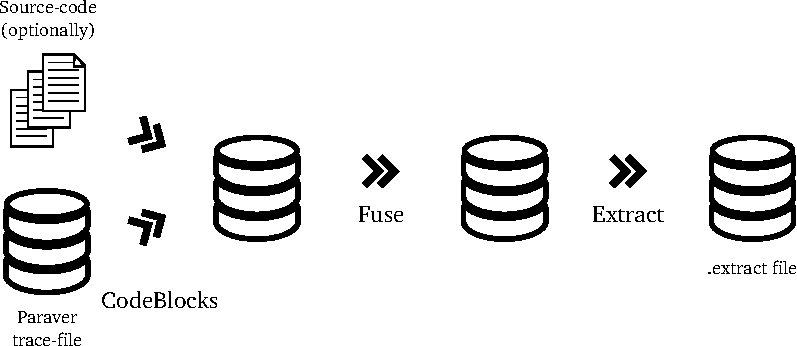
\includegraphics[width=0.5\textwidth]{figures/user-guide/codeblocks-fuse-extract.pdf}
  \caption{Data-flow for the first component of the folding.}
  \label{fig:dataflow_1st_component_folding}
\end{figure}


The first component is divided into three phases that are executed one after another with the user-given trace-file and each of these parse the given trace-file and generates another trace-file that will be used in the subsequent phase as depicted in Figure~\ref{fig:dataflow_1st_component_folding}.
Each of these phases are built in a similar fashion.
They parse the input trace-file and keep in memory information regarding the thread state, and eventually, add information to the output.
The phases are:

\begin{enumerate}

	\item \texttt{codeblocks} (found in \texttt{src/codeblocks})\\
	This phase attributes to each sample information regarding to the loop / code region that it belongs to according to the application source code. 

	\item \texttt{fuse} (found in \texttt{src/fuse})\\
	This phase compacts the trace-file and ensures that the resulting trace-file is well formed.

	\item \texttt{extract} (found in \texttt{src/extract})\\
	This is the final phase and extracts information regarding the instances and samples within the trace-file.

\end{enumerate}

The output of this component is a set of files containing information relative to the application. 
The most notable output is the \texttt{.extract} file, which contains the sequence of instances and their samples.
For instance, Listing~\ref{lst:ExampleGenerationInterpolationOutput} shows the contents of the \texttt{.extract} file generated using the provided example to demonstrate the API facility.
This listing contains information regarding one instance of the \texttt{FunctionA} region.
The instance starts at timestamp 1,000~ns and lasts 4,500~ns, and it executes up to 2,500 instructions (PAPI\_TOT\_INS) and takes 5,000 cycles (PAPI\_TOT\_CYC) to complete.
This instance has two samples associated that ocurred at timestamps 2,000 and 4,000, and each of those provides information regarding the aforementioned performance counters.

\begin{lstlisting}[
 frame=tb,
 basicstyle=\small\ttfamily,
 keywordstyle=\small\bfseries,
 commentstyle=\small\itshape,
 numbers=left,
 firstnumber=1,
 numberstyle=\tiny\color{gray},
 captionpos=t,
 caption={Output example for the extract phase of the \FOLDING mechanism.},
 tabsize=4,
 label=lst:ExampleGenerationInterpolationOutput,
 float=h
]
I 2 2 2 FunctionA 1000 4500 2 PAPI_TOT_CYC 5000 PAPI_TOT_INS 2500
S 2000 1000 2 PAPI_TOT_CYC 2000 PAPI_TOT_INS 1000 0 0
S 4000 3000 2 PAPI_TOT_CYC 4000 PAPI_TOT_INS 2000 2 0 1 2 3 1 3 4 5 0
\end{lstlisting}


\section{Second component: applying the folding}

The main objective of this component relies on processing the instances and samples extracted and generate the output results.
These results include the temporal evolution of the performance counters, any models requested by the user, the source code references and memory references progression, and the results are written in gnuplot and \PARAVER trace files.
This section gives a summarized view of the folding work-flow by depicting the most notable class diagrams found in the application source code.

\begin{figure}
  \centering
  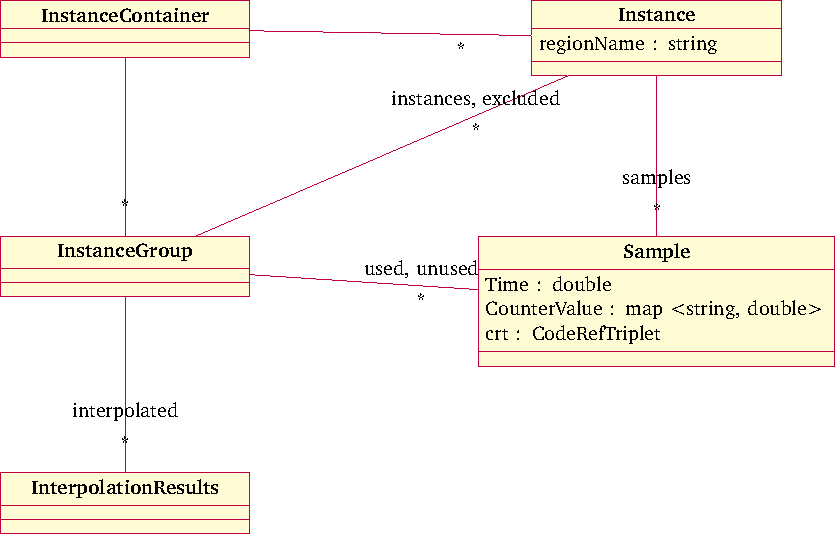
\includegraphics[width=0.80\textwidth]{figures/user-guide/tool-design-interpolate-instances.pdf}
  \caption{Main instances and samples related diagram classes.}
  \label{fig:tool_design_interpolate_instances}
\end{figure}


Figure~\ref{fig:tool_design_interpolate_instances} shows a portion of the classes that are most important within this tool.
The classes \textsl{Instance} and \textsl{Sample} refer to the instances and samples as-is, without any further processing and as generated by the \texttt{extract} tool, in which each \textsl{Instance} contains a set of \textsl{Sample}, and every \textsl{Instance} belongs to an \textsl{InstanceContainer}.

\documentclass{standalone}

\usepackage{tikz}
\usepackage{pgf-umlcd}
\usepackage[bitstream-charter]{mathdesign} % +1! taules mes petites i hi caben
\usepackage[T1]{fontenc}
\usepackage[utf8]{inputenc}

\begin{document}

\begin{tikzpicture}

\begin{abstractclass}[text width=6cm]{InstanceSeparator}{0,0}
\operation{InstanceSeparator (bool keepallgroups);}
\operation[0]{separateInGroups (vector<Instance>);}
\end{abstractclass}

\begin{class}[text width=5cm]{InstanceSeparatorAuto}{-6,-4}
\inherit{InstanceSeparator}
\end{class}
\begin{class}[text width=5cm]{InstanceSeparatorDBSCAN}{0,-4}
\inherit{InstanceSeparator}
\end{class}
\begin{class}[text width=5cm]{InstanceSeparatorNone}{6,-4}
\inherit{InstanceSeparator}
\end{class}
\end{tikzpicture}

\end{document}


After reading every \textsl{Instance}, the folding may apply a clustering algorithm (see Figure~\ref{fig:tool_design_interpolate_instance_separator}) according to the duration of each instance in order to reduce the difference between folded \textsl{Instance}.
Currently, there are three alternatives regarding the grouping.

\begin{itemize}

	\item \textsl{InstanceSeparatorNone} groups all instances into a single group.

	\item \textsl{InstanceSeparatorAuto} automatically groups the instances according to their duration. The grouping partitions the time-space interval defined by the shortest and longest instances and looks for group of nearby instances.

	\item \textsl{InstanceSeparatorDBSCAN} groups the instances according to a DBSCAN algorithm applied to the duration of the instances. The DBSCAN algorithm groups together instances that are closely packed together (instances with many nearby neighbors) in terms of time and marks as outliers those instances that lie alone in low-density regions. This grouping uses the ClusteringSuite implementation from the BSC performance tools\footnote{See \url{http://www.bsc.es/computer-sciences/performance-tools/downloads}.}.

\end{itemize}

This grouping begets the \textsl{InstanceGroup} objects which contains references to those \textsl{Instance} that belong to that particular group.
Then, the folding removes the outliers to each \textsl{Instance} within every \textsl{InstanceGroup} and store the outliers and the remaining in the \textit{excluded} and \textit{instances} associations, respectively.

\documentclass{standalone}

\usepackage{tikz}
\usepackage{pgf-umlcd}
\usepackage[bitstream-charter]{mathdesign} % +1! taules mes petites i hi caben
\usepackage[T1]{fontenc}
\usepackage[utf8]{inputenc}

\begin{document}

\begin{tikzpicture}

\begin{abstractclass}[text width=8cm]{SampleSelector}{0,0}
\operation[0]{select (InstanceGroup, vector<string> Counters);}
\end{abstractclass}

\begin{class}[text width=4cm]{SampleSelectorDefault}{-5,-4}
\inherit{SampleSelector}
\end{class}
\begin{class}[text width=4cm]{SampleSelectorFirst}{0,-4}
\inherit{SampleSelector}
\end{class}
\begin{class}[text width=4cm]{SampleSelectorDistance}{5,-4}
\inherit{SampleSelector}
\end{class}
\end{tikzpicture}

\end{document}


Since the complexity of the contouring algorithms depends on the number of points to connect, and therefore the number of samples to fold, the \FOLDING tool supports limiting the number of samples given to these algorithms.
Figure~\ref{fig:tool_design_interpolate_sample_selector} depicts the class diagram of the available \textsl{SampleSelector} mechanisms to limit the number of samples.

\begin{itemize}

	\item \textsl{SampleSelectorDefault} the \textit{select} method returns all of the samples within the \textsl{InstanceGroup}. This is useful when the user does not impose any limit to the number of samples to be folded.

	\item \textsl{SampleSelectorFirst} receives a threshold ($N$) in the class constructor. Then, the \textit{select} method tags the first $N$ samples for the processing while the rest are marked as \textit{unused}.

	\item \textsl{SampleSelectorDistance} receives a threshold ($N$) in the class constructor. Then, the \textit{select} method tags $N$ samples that are equidistant within the \textsl{Instance} duration, while the rest are \textit{unused}.

\end{itemize}

\begin{figure}
  \centering
  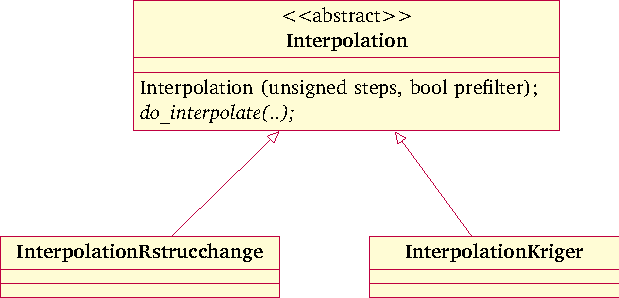
\includegraphics[width=0.50\textwidth]{figures/user-guide/tool-design-interpolate-interpolation.pdf}
  \caption{Performance counter interpolation related diagram classes.}
  \label{fig:tool_design_interpolate_interpolation}
\end{figure}


Then the \FOLDING repeatedly applies the contouring algorithm to the \textit{used} samples among the different \textsl{InstanceGroup} objects.
The contouring algorithm applies to each performance counter individually, and as of writing this document, there are two approaches that honor the \textsl{Interpolation} super-class virtual method (mainly \texttt{do\_interpolate}):

\begin{itemize}

	\item \textsl{InterpolationKriger} uses the self-provided contouring algorithm based on the Kriging mechanism to implement the \texttt{do\_interpolate}.

	\item \textsl{InterpolationRstrucchange} employs the strucchange package\footnote{\url{http://cran.r-project.org/web/packages/strucchange/index.html}} from the R statistical package\footnote{\url{http://www.r-project.org}} to use piece-wise linear regressions to the folded samples. Additionally, this package may benefit from parallel environments if the doParallel package\footnote{\url{http://cran.r-project.org/package=doParallel}} is available on the system.

\end{itemize}

The interpolation results are stored, per performance counter, into \textsl{InterpolationResults} objects that are associated by \textsl{InstanceGroup} by the attribute \textit{interpolated} (as depicted in Figure~\ref{fig:tool_design_interpolate_instances}).
The \textit{interpolated} attribute is implemented as a hash function indexed by the performance counter, so that the interpolation results can be fetched easily.

\documentclass{standalone}

\usepackage{tikz}
\usepackage{pgf-umlcd}
\usepackage[bitstream-charter]{mathdesign} % +1! taules mes petites i hi caben
\usepackage[T1]{fontenc}
\usepackage[utf8]{inputenc}

\begin{document}

\begin{tikzpicture}

\begin{abstractclass}[text width=5cm]{ComponentNode}{0,0}
\operation[0]{evaluate (InterpolationResults);}
\end{abstractclass}

\begin{class}[text width=4cm]{ComponentNode-constant}{-5,-4}
\inherit{ComponentNode}
\end{class}
\begin{class}[text width=4cm]{ComponentNode-data}{0,-4}
\inherit{ComponentNode}
\end{class}
\begin{class}[text width=4cm]{ComponentNode-derived}{5,-4}
\inherit{ComponentNode}
\end{class}

\association{ComponentNode-derived}{}{}{ComponentNode}{children}{2};

\begin{class}[text width=5cm]{ComponentModel}{8,0}
\end{class}

\association{ComponentModel}{}{}{ComponentNode}{}{1}

\begin{class}[text width=5cm]{Model}{8,4}
\operation{loadXML (file)}
\end{class}

\association{Model}{}{}{ComponentModel}{components}{*}

\end{tikzpicture}

\end{document}


\begin{lstlisting}[
 float=h,
 language=XML,
 frame=tb,
 basicstyle=\small\ttfamily,
 keywordstyle=\small\bfseries,
 commentstyle=\small\itshape,
 numbers=left,
 firstnumber=1,
 numberstyle=\tiny\color{gray},
 captionpos=t,
 caption={Folding example model that generates the L1D and L2D misses per instruction, in addition to the MIPS rate},
 label=lst:Folding_sample_model,
]
<?xml version='1.0'?>

<model name="sample" title-name="Sample model"
       y1="Ratios" y2="MIPS" y1-stacked="no">

    <component name="l1_dcm_ratio" title-name="L1 DCM" where="y1"
               color="red">
        <operation type='/'>
            <value> PAPI_L1_DCM </value>
            <value> PAPI_TOT_INS </value>
        </operation>
    </component>

    <component name="l2_dcm_ratio" title-name="L2 DCM" where="y1"
               color="blue">
        <operation type='/'>
            <value> PAPI_L2_DCM </value>
            <value> PAPI_TOT_INS </value>
        </operation>
    </component>

    <component name="mips" title-name="MIPS" where="y2" color="black">
        <value> PAPI_TOT_INS </value>
    </component>

</model>
\end{lstlisting}


The \FOLDING allows defining performance models based on performance counters using XML files (see Listing~\ref{lst:Folding_sample_model} for exemplification purposes and \texttt{\$\{FOLDING\_HOME\}/etc/models} for more detailed examples).
Within every XML there may be one or several components (in the last Listing these are: \texttt{l1\_dcm\_ratio}, \texttt{l2\_dcm\_ratio} and \texttt{mips}) that will be later represented in the resulting gnuplot using the selected colors and Y-axis (left [y1] or right [y2]).
Each component may refer to the instantaneous value of a certain performance counter (as in the \texttt{mips} component), a constant value or the operation (addition, subtraction, multiplication and division) between two other values (as in \texttt{l1\_dcm\_ratio} and \texttt{l2\_dcm\_ratio} components).
The \FOLDING implements the performance models based on performance counters employing the diagram classes show in Figure~\ref{fig:tool_design_interpolate_model}.
The XML model files are loaded into the \textsl{Model} class and each of them may contain multiple components (\textsl{ComponentModel}).
The \textsl{ComponentModel} implements the definition of the component on top of the \textsl{ComponentNode} derived sub-classes.
These sub-classes allow referencing constant values (\textsl{ComponentNode\_constant}), interpolated results from a specific performance counter (\textsl{ComponentNode\_data}) and operation between other two \textsl{ComponentNode} objects).

\begin{figure}
  \centering
  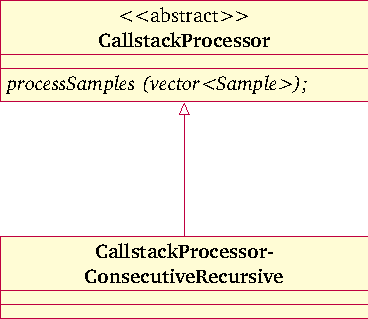
\includegraphics[width=0.35\textwidth]{figures/user-guide/tool-design-interpolate-callstack-processor.pdf}
  \caption{Call-stack processing related diagram classes.}
  \label{fig:tool_design_interpolate_callstackprocessor}
\end{figure}


With respect to the analysis of the call-stack, the \FOLDING tool has implemented this analysis through the \textsl{CallstackProcessor} related-classes that receives a set of \textsl{Sample} objects to explore.
Currently, the unique implementation available relies on aligning the call-stacks from the given samples and then exploring the call-stack frames at a given level whether consecutive samples refer to the same routine.
If the number of samples surpasses a given threshold, then applies it recursively to the next level until no more levels are available or the number of samples do not surpass the threshold.


\chapter{API}

This section covers the public API available in the \FOLDING package.
This API is meant to allow the \FOLDING tool to interact with other performance analysis tools in addition to \EXTRAE.

\section{Generation of input files for the \FOLDING}

\subsection{Usage example}

The directory \texttt{\$FOLDING\_HOME/share/examples/folding-writer} contains an example that shows how to generate an input file for the folding from a programatically point of view.
The example can be compiled using the following command:

\begin{verbatim}
# cd $FOLDING_HOME/share/examples/folding-writer
# make
\end{verbatim}

The Listing~\ref{lst:ExampleGenerationInterpolation} shows the example provided in the distributed/installed package.
This example demonstrates how to programatically create an \texttt{.extract} file for the \texttt{interpolate} binary of the \FOLDING package.

\begin{lstlisting}[
 language=C++,
 frame=tb,
 basicstyle=\footnotesize\ttfamily,
 keywordstyle=\footnotesize\bfseries,
 commentstyle=\footnotesize\itshape,
 numbers=left,
 firstnumber=1,
 numberstyle=\tiny\color{gray},
 captionpos=t,
 caption={Example of generating an input file for the \FOLDING mechanism.},
 tabsize=4,
 label=lst:ExampleGenerationInterpolation,
]
/*****************************************************************************\
 *                        ANALYSIS PERFORMANCE TOOLS                         *
 *                                   Folding                                 *
 *              Instrumentation package for parallel applications            *
 *****************************************************************************
 *     ___     This library is free software; you can redistribute it and/or *
 *    /  __         modify it under the terms of the GNU LGPL as published   *
 *   /  /  _____    by the Free Software Foundation; either version 2.1      *
 *  /  /  /     \   of the License, or (at your option) any later version.   *
 * (  (  ( B S C )                                                           *
 *  \  \  \_____/   This library is distributed in hope that it will be      *
 *   \  \__         useful but WITHOUT ANY WARRANTY; without even the        *
 *    \___          implied warranty of MERCHANTABILITY or FITNESS FOR A     *
 *                  PARTICULAR PURPOSE. See the GNU LGPL for more details.   *
 *                                                                           *
 * You should have received a copy of the GNU Lesser General Public License  *
 * along with this library; if not, write to the Free Software Foundation,   *
 * Inc., 51 Franklin Street, Fifth Floor, Boston, MA 02110-1301 USA          *
 * The GNU LEsser General Public License is contained in the file COPYING.   *
 *                                 ---------                                 *
 *   Barcelona Supercomputing Center - Centro Nacional de Supercomputacion   *
\*****************************************************************************/

#include "folding-writer.H"
#include <fstream>

using namespace std;

int main (int argc, char *argv[])
{
	string nameRegion = "FunctionA";
	unsigned long long startRegion = 1000;
	unsigned long long durationRegion = 4500;

	/* NOTE:: Counters are given in deltas from their previous read, not as absolute values */
	map<string, unsigned long long> c1;
	c1["PAPI_TOT_INS"] = 1000;
	c1["PAPI_TOT_CYC"] = 2000;
	map<unsigned, CodeRefTriplet> crt1;
	Sample *s1 = new Sample (2000, 2000-startRegion, c1, crt1);

	map<string, unsigned long long> c2;
	c2["PAPI_TOT_INS"] = 1000;
	c2["PAPI_TOT_CYC"] = 2000;
	map<unsigned, CodeRefTriplet> crt2;
	CodeRefTriplet codeinfo_l0 (1,2,3);
	CodeRefTriplet codeinfo_l1 (3,4,5);
	crt2[0] = codeinfo_l0;
	crt2[1] = codeinfo_l1;
	Sample *s2 = new Sample (4000, 4000-startRegion, c2, crt2);

	/* Last sample typically coincides with end of region -- see durationRegion,
	   Folding::Write won't emit in a S entry */
	map<string, unsigned long long> c3;
	c3["PAPI_TOT_INS"] = 500;
	c3["PAPI_TOT_CYC"] = 1000;
	map<unsigned, CodeRefTriplet> crt3;
	Sample *s3 = new Sample (4500, 4500-startRegion, c3, crt3);

	vector<Sample*> vs;
	vs.push_back (s1);
	vs.push_back (s2);
	vs.push_back (s3);

	ofstream f("output.extract");
	if (f.is_open())
	{
		FoldingWriter::Write (f, nameRegion, 1, 1, 1, startRegion,
		  durationRegion, vs);
		f.close();
	}

	return 0;
}
\end{lstlisting}


The given example considers that the region \texttt{FunctionA} has been identified somehow by the underlying monitoring mechanism, starts at 1,000~ns and lasts 4,500~ns (lines 31-33).
Within this period of time, three samples have occurred (\textit{s1-s3}, created in lines 40, 50 and 58, respectively).
Samples contain performance counter information and source code references.
The performance counter information is given in a relative manner, thus each sample contains the difference from the previous sample (or starting point).
For instance, sample \textit{s1} captured information from two performance counters (\texttt{PAPI\_TOT\_INS} and \texttt{PAPI\_TOT\_CYC}) that counted 1,000 and 2,000 events since the start of the region at time-stamp 2,000~ns (lines 36-40).
The second sample (\textit{s2}) does not only contain information from performance counters, but also contains a call-stack segment referencing two call-stack frames.
The first frame (\texttt{codeinfo\_l0}) refers to the routine coded as 1, which has source code information coded as 2, and AST-block information coded as 3 (line 46).
The same applies to second frame (\texttt{codeinfo\_l1}) - (line 47).
These frames are mapped into depths 0 and 1 (where 0 refers to the top of the call-stack) in lines 48 and 49, and then the sample is built using the performance counter information and the call-stack information in line 50.
Finally, the last sample (\textit{s3}) only accounted 500 and 1,000 events for the \texttt{PAPI\_TOT\_INS} and \texttt{PAPI\_TOT\_CYC} performance counters respectively, but did not capture any source code reference (lines 54-58).
This last sample should coincide with the end of the region (\texttt{FunctionA}), and may not be necessarily information captured from a sample point, but from an instrumentation point that indicates the end of the region.
All these samples are packed together in a STL vector container (lines 60-63), and then the \texttt{FoldingWriter::Write} static method dumps all the information from the samples using the given output stream (lines 65-71).



\end{document}


